\section{Reconstruction of Collision Events in the ATLAS Detector}%
\label{sec:object_reco_at_atlas}

\todo[inline]{Introductory sentence}


\subsection{Tracking and Vertexing}

The reconstruction of trajectories of charged particles is referred to as track
reconstruction or tracking. The inputs to the track reconstruction in the ID of
the ATLAS detector are \emph{space-points} from the pixel and SCT detector, and
\emph{drift circles} from the TRT. Space-points are measurements of location in
three-dimensional space obtained by clustering the charge signals of adjacent
segments in the pixel and SCT detectors. Drift circles are measurements of
distance from the anode wires of individual straw-tubes in the TRT obtained from
measured electron drift times in the straw-tubes.

Track reconstruction employs pattern recognition techniques to select
space-points and drift circles that are compatible with the hypothesis of a
charged particle in the axial magnetic field of the ID. Least-squares fits are
performed, using selected space-points and drift circles, to determine the
parameters characterising the track at a reference point. This reference point
is the point of closest approach (perigee) to the nominal beamspot
position.\footnote{Once the PV is reconstructed, the perigee with respect to the
  PV is often used.} Five parameters are sufficient to describe the track at the
perigee. The transverse (longitudinal) distance of the perigee from the
reference point given by $d_0$ ($z_0$), also referred to as the transverse
(longitudinal) impact parameter of the track. The azimuthal and polar angle of
the track at the perigee given by $\phi$ and $\theta$, respectively. Finally,
the ratio of electric charge and transverse momentum, $q / \pT$, a measure of
the curvature of the track.

At the ATLAS experiment, two primary tracking algorithms are used which are
referred to as the \emph{inside-out} and \emph{outside-in}
algorithms~\cite{Cornelissen:2007vba,Salzburger:2015sgq,PERF-2015-08}. The
inside-out algorithm starts by reconstructing tracks in the pixel and SCT
detector only, which are optionally extended to the TRT. The outside-in
algorithm starts with reconstructing track segments in the TRT which are then
combined with space-points from the pixel and SCT detectors. The outside-in
algorithm is meant to recover tracks from secondary charged particles such as
decay products of $b$-hadrons.

Vertex reconstruction~\cite{PERF-2015-01}


% Two main tracking algorithms are used by the ATLAS
% experiment, \emph{inside-out} and \emph{outside-in}
% algorithm~\cite{Cornelissen:2007vba,Salzburger:2015sgq,PERF-2015-08}:
% \begin{description}

% \item[Inside-out algorithm] The inside-out algorithm starts by finding track
%   seeds in the pixel and SCT detector. Track seeds are short track candidate
%   segments constructed from three space-points in the ID. These track seeds are
%   used as a starting point for an iterative track fit using a Kalman
%   filter~\cite{Fruhwirth:1987fm} extending the track candidates with
%   space-points of increasing radius (inside-out). An ambiguity resolution step,
%   see for example Ref.~\cite{PERF-2015-08}, is applied on all track candidates
%   to remove tracks from combinations of unrelated space-points and track
%   duplicates.

%   Moreover, a precision fit is performed...  \todo[inline]{TRT extension?}

% \item[Outside-in algorithm] The outside-in algorithm is used to recover
%   efficiencies for non-promptly produced charged particles (e.g.\ secondary
%   particles from $b$-hadron decays) which might not have a corresponding track
%   seed.

% \end{description}


% https://cds.cern.ch/record/2018442/files/pdf.pdf

% - formation of localised clusters of charge depositions in the silicon detectors
% -> three-dimensional space-points

% - drift circles for the TRT

% - inside-out:
% 1. Seeding from three space points
% 2. Combinatorial Kalman filter builds first track candidates
% 3. Resolution of ambiguities and application of quality cuts
% 4. Track fit:

% - outside-in:
% -> If no track seed exists (e.g. tracks from secondary vertices) -> start in the TRT and go inwards




\subsection{Topological Clustering of Energy in Calorimeter Cells}

\subsection{Electrons}

\subsection{Muons}

\subsection{Jets and $b$-tagging}

\subsection{Hadronic Decays of Tau Leptons}

\begin{figure}[htb]
  \begin{subfigure}[b]{0.47\textwidth}
    \centering

    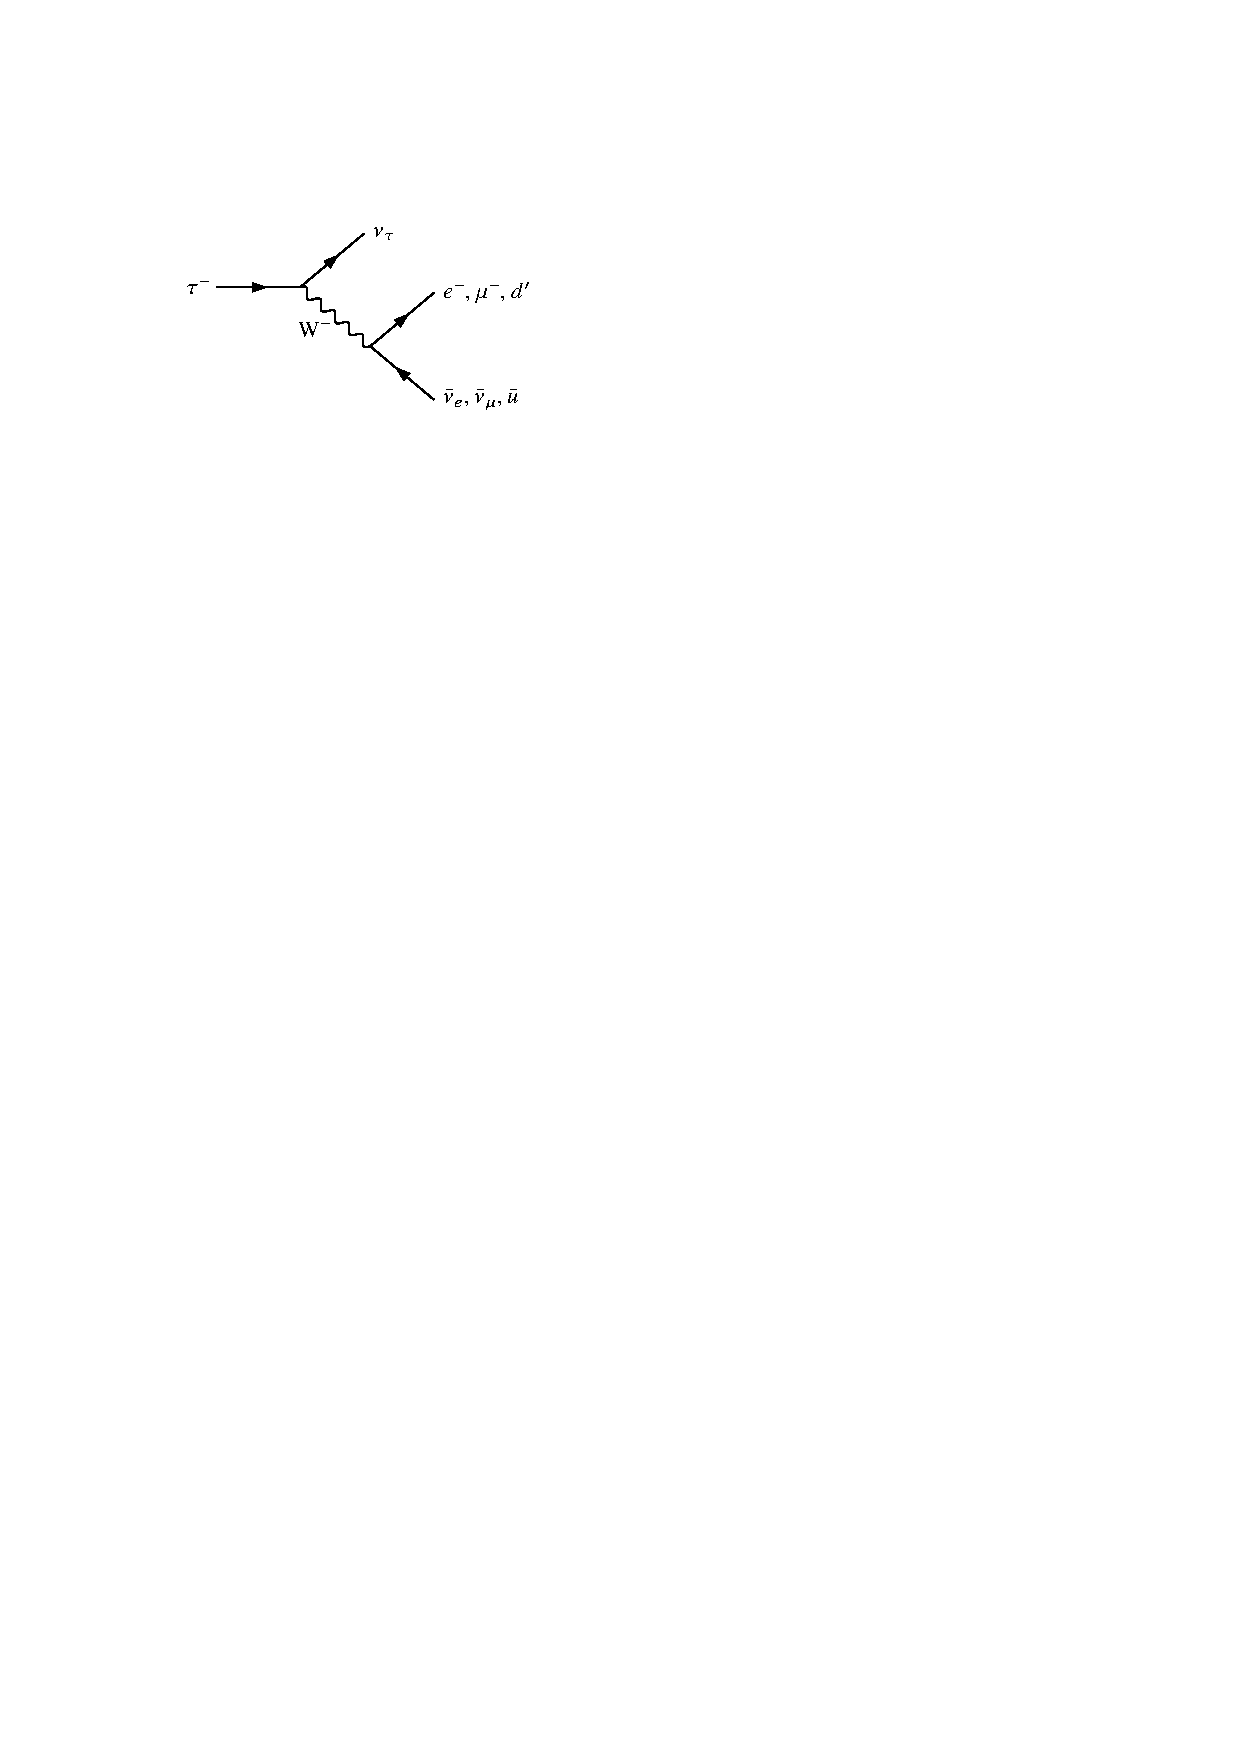
\includegraphics{figs/tauid/tau_decay_feynman}

    \vspace*{3em}
    \subcaption{a}%
    \label{fig:tau_feynman}
  \end{subfigure}\hfill
  \begin{subfigure}[b]{0.47\textwidth}
    \centering

    \begin{overpic}[scale=0.9]{figs/tauid/tau_branching_pie_chart}
      \put (31, 83) {$\pi^- \nu_\tau$}
      \put (-5.5, 45) {$\pi^- \pi^0 \nu_\tau$}
      \put (16, 7) {$\pi^- 2 \pi^0 \nu_\tau$}
      \put (40.5, 2) {$2 \pi^- \pi^+ \nu_\tau$}
      \put (65, 6.5) {$2 \pi^- \pi^+ \pi^0 \nu_\tau$}
      \put (76.5, 15.5) {other}
      \put (70, 77.5) {$e^- \bar{\nu}_e \nu_\tau$}
      \put (88.5, 41.5) {$\mu^- \bar{\nu}_\mu \nu_\tau$}
    \end{overpic}

    \subcaption{}%
    \label{fig:tau_branching_ratios}
  \end{subfigure}
  \caption{Decay and branching ratios of the tau
    lepton. Charge-conjugate decay modes are omitted.}
\end{figure}


\subsubsection{Seed Jet}

Seeded with AntiKt 0.4 jets on TopoClusters at the LC scale.

\subsubsection{Tau Vertex Association}

TJVA

\subsubsection{Track Association}

\cite{duschinger}

\todo[inline]{Make sure to point out the difference between ``tau
  tracks'' and all other tracks.}

\subsubsection{Energy Calibration}

MVA TES

\subsubsection{Electron Veto}
\subsubsection{Tau Identification}

\subsection{Missing Transverse Energy}%
\label{sec:atlas_met}


%%% Local Variables:
%%% mode: latex
%%% TeX-master: "../../phd_thesis"
%%% End:
